\section{Terminales}
Los terminales son los subsistemas expuestos al campo, cada uno representa un punto de acceso. A diferencia del servidor, que es único, el sistema se compone de varios terminales en cada punto de acceso, en este caso tres, pero en una aplicación similar el número de terminales podría extenderse. Por este motivo, los terminales fueron diseñados para ser fácilmente replicables, adaptables y de bajo costo, dado que el costo total del sistema aumenta de marginalmente con cada nueva unidad incorporada.


\subsection{Selección de hardware}
Un terminal se compone de un microcontrolador, diversos módulos electrónicos y dispositivos de interfaz con el entorno físico. Entre ellos se encuentran:
\begin{itemize}
    \item Una cámara
    \item Un sensor NFC
    \item Un tranceiver RS-485
    \item Una antena WiFi
    \item Dos relés, uno para permitir el ingreso destrabando la puerta y otro para hacer sonar el timbre
    \item Un interruptor, para que los visitantes externos soliciten el acceso
\end{itemize}

La primera opción para utilizar como controlador principal del proyecto, fue el kit de desarrollo ESP32-CAM, basado en el módulo WROM-32, el cual integra un microcontrolador ESP32 junto con una antena de radio e interfaces para conectividades WiFi, Bluetooth entre otras, con la particularidad de que incluye un socket para conectar una cámara, por ejemplo la OV2640 que viene incluida. El mayor problema del módulo, es la limitada cantidad de pines GPIO disponibles y utilizables, haciendo poco viable para ser el controlador principal del terminal, a pesar de ser computacionalmente capaz de cumplir con las funciones requeridas.

Se optó por una arquitectura distribuida, en la que el ESP32-CAM queda dedicado exclusivamente a la adquisición y transmisión de imágenes, mientras que el procesamiento principal y el control de los periféricos recaen sobre un segundo ESP32.

\subsubsection{Microcontrolador}
El ESP32 fue seleccionado por ofrecer un adecuado equilibrio entre capacidad de procesamiento, memoria, periféricos integrados y costo, además de incorporar múltiples interfaces de comunicación (UART, SPI, I²C, WiFi y Bluetooth). 
Otra ventaja es su procesador de doble núcleo que permite multitasking real.
Para el prototipo se utilizará un kit de desarrollo ESP32 DEV KIT V1, pudiéndose reemplazar en producción por el microcontrolador suelto, ya que esta etapa del sistema no requiere conectividad WiFi.

\subsubsection{Cámara}
Para el prototipo se optó, como ya se mencionó anteriormente en el uso del kit de desarrollo ESP32 CAM, el cual se vende con la cámara OV2640.
Esta elección se basa en el fácil  acceso y el bajo precio del módulo, el cual resuelve varios aspectos de la toma y transmisión de fotografías. 
La cámara cuenta con una resolución de 2 MP, suficiente para un reconocimiento de un rostro por parte de un validador humano. El módulo además incorpora un led de alta luminosidad que funciona como flash de la cámara, y una memoria PSRAM externa de 4 MB que permite almacenar temporalmente las imágenes.
La conectividad WiFi incorporada se utiliza para transmitir las imágenes al servidor mediante el protocolo HTTP.

Se comunica contra el microcontrolador principal mediante UART para recibir comandos y compartir información.

\subsubsection{Comunicación RS-485}
Para la comunicación con el servidor, el ESP32 debe comunicarse con un transreceptor que \enquote{traduzca} UART a 485. Se seleccionó un módulo basado en el circuito integrado MAX485, ampliamente utilizado para la conversión entre UART y RS-485.

\subsubsection{Lector NFC}
Para la lectura y escritura de las credenciales se seleccionó un módulo basado en el circuito integrado PN532 de NXP. Este dispositivo implementa internamente los protocolos necesarios para la comunicación con etiquetas RFID/NFC de alta frecuencia compatibles, proporcionando una interfaz de programación de alto nivel que simplifica el desarrollo del firmware. Asimismo, ofrece soporte para operaciones de lectura, escritura y autenticación sobre las etiquetas empleadas en el sistema.

Para este desarrollo se optó por las etiquetas NTAG-21X como credenciales de acceso.

El módulo cuenta con interfaz SPI para comunicarse con el controlador principal.

\subsubsection{Interfaces de campo}
Para la activación del timbre y el desbloqueo de la puerta se incorporan sendos relés en cada terminal, comandados por salidas digitales del controlador. Ambos equipos operan con tensión de red de 220 V CA.
Para el pulsador del timbre, se conectó entre GND y la entrada digital del ESP32 una bornera, que permita aprovechar el pulsador ya existente en la instalación.

\subsubsection{Alimentación}
Las ESP32 operan a 3,3 V, pero pueden alimentarse con 5 V, ya que las placas cuentan con reguladores de voltaje LDO incorporadas. El PN532 también cuenta con un regulador y tanto el transceptor como los relés se deben alimentar con 5 V. Se propone entonces alimentar mediante un conector micro USB tipo A (u opcionalmente un tipo C), para poder alimentar el circuito desde una fuente externa, como por ejemplo un cargador de teléfono celular.
Se añade además un capacitor de 470~$\mu$F para mitigar los picos de consumo de corriente que se producen durante el encendido de la cámara o de la interfaz WiFi.

\subsection{Firmware del controlador}
Para programar el firmware del controlador, se utilizó el framework oficial de Espressif, ESP IDF, a través de la extensión del entorno Visual Studio Code.
Dado que el controlador debe ejecutar de forma concurrente tareas de comunicación, adquisición de datos, procesamiento y control de dispositivos externos, se optó por desarrollar el firmware utilizando el sistema operativo de tiempo real FreeRTOS, el cual se incorpora en forma nativa en el sdk de ESP32, por lo que la integración es orgánica.

\subsubsection{Sistemas operativos en tiempo real}

Una aplicación bare-metal suele organizarse alrededor de un lazo principal (superloop) que ejecuta secuencialmente todas las funciones del sistema. En cambio, un RTOS permite dividir la aplicación en múltiples tareas concurrentes, administradas por un planificador que decide cuál debe ejecutarse en cada instante. En FreeRTOS una tarea corresponde a una función independiente, normalmente implementada como un bucle infinito, aunque puede finalizar cuando su ejecución concluye. La ejecución de las tareas se alternan orquestada por el \enquote{scheduler} o planificador.

Esta arquitectura permite modularizar el código, asignar prioridades y encapsular las responsabilidades.

Otra  funcionalidad de los RTOS es, como su nombre lo indica, la posibilidad de asegurar la ejecución de ciertos ciclos con limitaciones de tiempo real, aunque en esta aplicación los requisitos temporales no son estrictos.


Las tareas pueden encontrarse en cuatro distintos estados:

\begin{itemize}
    \item \textbf{Running} o corriendo, la tarea se está ejecutando.
    \item \textbf{Ready} o lista, la tarea está lista para ejecutarse, pero la cpu está tomada por otra tarea de mayor o igual prioridad.
    \item \textbf{Suspended} o suspendida, la tarea se encuentra \enquote{dormida}, es decir temporalmente desactivada, solo puede ser reactivada por otra tarea.
    \item \textbf{Blocked} o bloqueada, la tarea está esperando a un evento para estar lista.
\end{itemize}
Solo las tareas en estado Running consumen ciclos de CPU, por lo que se dice que los demás estados componen un \enquote{superestado} llamado Not Running.

Para definir cuál tarea de todas las que están listas se ejecuta hay dos formas de trabajar, la operación colaborativa, donde cada tarea cede el procesador en determinado momento, y la operación apropiativa, donde el scheduler interrumpe una tarea para darle CPU a otra. FreeRTOS para ESP-IDF utiliza planificación apropiativa basada en prioridades.

La apropiación puede ser para ejecutar una tarea de mayor prioridad o bien para alternar entre varias tareas de igual prioridad.

La suspensión se da cuando una tarea debe dejar de ejecutarse temporalmente, una tarea puede suspenderse a sí misma y a otras, pero solo puede ser retomada desde otra tarea.

El bloqueo se da cuando una tarea debe esperar un evento para continuar su ejecución, tal como la finalización de un timer, el cambio de una bandera o bien el aviso de otra tarea. La espera de una interrupción no puede bloquear directamente a una tarea, pero puede enviarse el aviso de desbloqueo desde el callback de dicha interrupción.

 \begin{figure}[t]
	\centering
	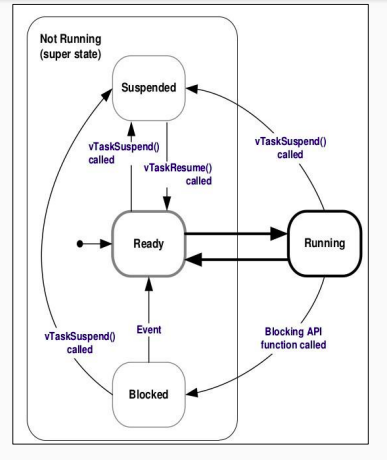
\includegraphics[width=0.8\textwidth]{img/MEF_RTOS.png}
	\caption{Diagrama de estados de una tarea en un RTOS}
	\label{fig:MEF_RTOS}
\end{figure}


Las tareas interactúan entre sí mediante herramientas de comunicación y de sincronismo.

Las principales herramientas de sincronismo son los semáforos. Un semáforo contiene un contador. \enquote{Ceder} o \enquote{dar} un semáforo aumenta el contador y tomarlo lo disminuye, si se intenta tomar un semáforo que está en cero, la tarea se bloquea. 

Un caso particular es el semáforo binario, el cual solo puede aumentar hasta uno, es decir, reconoce dos estados. Es particularmente útil para desbloquear una tarea desde otra de forma genérica.

Un caso particular del semáforo binario es el semáforo de exclusión mutua o \enquote{mutex}, el cual solo puede ser retornado por la misma tarea que lo tomó, se utiliza para proteger espacios de memoria de una escritura por parte de otra tarea, pudiendo dejar los datos compartidos en un estado inconsistente.

Otro método de sincronismo es la notificación, la cual es más rápida y eficiente que el semáforo binario, pero sirve solo para notificar una tarea en específico.

Las estructuras de comunicación tienen como funcionalidad principal enviar datos de una tarea a la otra, aunque también pueden utilizarse para la sincronización.
Ejemplos de estas estructuras son el \textit{stream buffer}, el cual transmite  cadenas de bytes enteros de longitud variable, ideal para flujo continuo de datos, el \textit{message buffer}, el cual envía mensajes de bytes enteros de longitud definida, mejor para datos ya filtrados, y la \textit{queue} o cola de mensajes, la cual puede transmitir elementos de tamaño definido, por ejemplo estructuras de datos.


\subsubsection{Comunicación con el servidor}
Para comunicar el controlador con el servidor se seleccionó, en la capa física del modelo OSI el protocolo serial RS-485 como ya se indicó. El transreceptor \enquote{traduce} las señales diferenciales al protocolo UART por el cual se comunica el microcontrolador. 

Para el microcontrolador se desarrollaron dos librerías que gestionen la comunicación.
La primera, llamada \textit{app\_uart} se ubica en la capa de enlace de datos y se ocupa de gestionar la recepción y el envío de tramas crudas, sin ningún tipo de procesamiento.
La segunda, llamada \textit{protocol}, se ubica en la capa de aplicación y le  corresponde procesar las tramas entrantes así como preparar las salientes.

Los datos entrantes son recibidos en una tarea dedicada de la librería \texttt{app\_uart} y cargados en un stream buffer, el cual debe ser leído por la tarea correspondiente de la librería del protocolo.

La librería \texttt{app\_uart} se compone de tres funciones y una tarea:

\begin{lstlisting}
void uart_init(void);
void uart_rx_task(void *pvParameters);

void app_uart_send(uint8_t *trama, int len);
StreamBufferHandle_t uart_get_rx_streambuffer(void);

\end{lstlisting}


La función de inicialización primero crea el stream buffer, el cual es local, por lo que para recuperar los datos se debe acceder a él mediante un \enquote{getter}, es decir una función pública que devuelve la estructura de datos.

Luego se configura la operación del periférico, basado en las guías de la documentación oficial y códigos de ejemplo, y luego adaptado a las necesidades de este proyecto.
Se crea una estructura de configuración donde se definen los parámetros de operación, se elimina el bit de paridad y el control de flujo por hardware, ya que el método de detección de errores se aplica en la capa de aplicación y el flujo se programa a mano.
La inicialización configura el puerto UART1 para trabajar en modo RS485 y reaccionando a eventos mediante interrupciones, todo esto de forma transparente al desarrollador.

Lo siguiente es instalar el driver, en este caso se definen los tamaños de los buffers de recepción y de transmisión (este último en 0). Estos buffers son \enquote{invisibles} para el programador, por ejemplo el buffer de recepción es circular y se va llenando con los bytes entrantes y vaciando con los que se leen explícitamente, el tamaño sirve para ver cuanto se pueden acumular. Se seteó en 2048 para asegurar el funcionamiento de forma conservadora, lo que se corresponde con más de 100 tramas de longitud máxima según se define en el protocolo.
El driver también se le carga una cola de eventos junto con su tamaño. Esto configura a la UART para trabajar por interrupciones que se ejecutan de forma transparente al usuario, cada vez que llegan datos, el sistema operativo interrumpe y carga en la cola un evento de bytes entrantes.

Posteriormente, se cargan las configuraciones de la estructura, y se setean los pines que se utilizaran. Finalmente, se establece el modo de trabajo, en este caso RS-485, que configura el pin antes definido como RTS para comandar el transceiver según la dirección de los datos. El pin restante es para control de flujo por hardware por lo que se deja sin usar.

La tarea \textit{uart\_rx\_task} reacciona a  los eventos y ante un evento del tipo UART\_DATA, pone los datos en un Stream Buffer static del archivo. Esto lo hace leyendo la cola de eventos.

La cola bloquea la tarea hasta la ocurrencia de un evento, en el caso de que el evento sea de datos se leen y se guardan en el buffer. Hay más tipos de eventos relativos a posibles fallos, como un desborde del buffer de recepción o bien problemas al recibir los datos. Se implementaron logs para estos casos sin desarrollar. Quedan como mejora futura el tratamiento de estos eventos cuando se acote el buffer de recepción y se suba la velocidad.

Para enviar los datos por uart se creó la función \textit{app\_uart\_send}, a la cual se le pasa como parámetro un puntero a un buffer (arreglo de enteros sin signo de 8 bits) y un campo de longitud.


La elección de esta arquitectura se debe a que la implementación del protocolo requiere que los datos entrantes se entreguen en un streambuffer y los salientes se reciban mediante un puntero. Manteniendo estas estructuras se podrían desarrollar librerías para que el protocolo opere con diferentes capas físicas, como por ejemplo CAN BUS.

\subsection{Protocolo Ramodbus}
La implementación de este módulo conllevó un doble desafío, primero la definición de un protocolo de capa de aplicación y segundo la implantación de este como librería, manteniendo robustez, desacoplamiento y portabilidad. Se decidió llamarlo \enquote{Ramodbus} por la inspiración a Modbus y el apellido del desarrollador.

Se evaluó utilizar Modbus RTU, dado que es un protocolo robusto, altamente probado y muy documentado con librerías en múltiples plataformas, además de estar diseñado para trabajar sobre RS-485.

La desventaja es que, al ser un protocolo pensado para comunicaciones con PLC's, hay que adaptar su uso a una aplicación IOT con otros comandos, otros tipos de datos, etc.
Se decidió entonces desarrollar un protocolo propietario inspirado en Modbus RTU pero adaptado a las necesidades de este proyecto, con la flexibilidad suficiente para ser reutilizado en aplicaciones similares. 

De Modbus RTU se mantienen las siguientes características:

\begin{itemize}
	\item Comunicación maestro - esclavo multipunto con múltiples esclavos
	\item Arbitraje mediante polling
	\item Funcionamiento en base a comandos
	\item Verificación de errores mediante CRC de 16 bits
\end{itemize}

La primera diferenciación viene de la complejidad de implementar un sincronismo temporal como Modbus RTU, en lugar de manejar los inicios y finales de trama mediante silencios y timeouts, se decidió incluir un byte de inicio de trama y un campo de longitud en el encabezado. De esta forma la trama queda de la siguiente manera:


\begin{center}
	\begin{bytefield}[bitwidth=0.6em]{32}

		
		% Fila 1: Encabezado estándar (4 bytes)
		\bitbox{8}{\footnotesize START} & 
		\bitbox{8}{\footnotesize NODO\_ID} & 
		\bitbox{8}{\footnotesize CMD} & 
		\bitbox{8}{\footnotesize LEN} 
		\bitbox{16}{\footnotesize PAYLOAD} & 
		\bitbox{16}{\footnotesize CRC16} \\
		%fila 2 ejemplo
		
		\bitbox{8}{\footnotesize 0xAA} & 
		\bitbox{8}{\footnotesize 0x0A} & 
		\bitbox{8}{\footnotesize 0x00} & 
		\bitbox{8}{\footnotesize 0x00} &
		\bitbox{16}{\footnotesize long variable} & 
		\bitbox{16}{\footnotesize 0x85 0x8C}
	\end{bytefield}
\end{center}



La principal innovación viene de los comandos, esta idea surgió en la etapa de implementación como método para optimizar la memoria reservada.
Como Modbus RTU es orientado a registros, tiene pocos comandos, pero siempre mantiene un payload mínimo, ya que requiere por ejemplo para encender una salida, la dirección de esta.

En una aplicación IOT se pueden tener funcionalidades muy simples que requieran solo de una orden, como por ejemplo encender el relé que desbloquea la puerta en este proyecto. Se decidió entonces que Ramodbus tenga tantos comandos como sea necesario. Para cada aplicación específica.

Esto determina en principio dos tipos de comandos: los obligatorios del protocolo y los comandos de la aplicación. Existen tres comandos obligatorios.

El comando 0x00 que del lado del maestro es un polling, una encuesta que pregunta al esclavo si hubo algún evento. En el caso de que el maestro requiera enviar un comando, simplemente reemplaza el comando de polling por el del comando. Desde el esclavo un comando 0x00 es un acknowledge (ACK).

El comportamiento del esclavo es responder de inmediato con los datos que tenga listos, si el maestro le pide datos, el esclavo probablemente responda con un ACK de inmediato y entregará los datos como respuesta a un ciclo de polling posterior. Esto puede parecer en principio una debilidad, porque se debe configurar el maestro para esperar las respuestas y confirmaciones por varios ciclos hasta considerar reenviar la solicitud. Sin embargo, esto trae una potencial mejora para aplicaciones críticas en tiempo con mayor número de esclavos, ya que al ofrecer una respuesta inmediata, se puede acelerar el ciclo de encuestas, incluso aprovechando el determinismo del RTOS. Esto es uno de los dos factores que tienen el potencial de compensar la diferencia de longitud en las tramas.

El segundo comando obligatorio es el 0x01, solo de parte del esclavo y representa el not-acknowledge (NACK), se dispara el  CRC se valida mal o si el campo len tiene un valor fuera de rango. Quedan a futuro posibilidades de agregarle más validaciones.

El tercer comando obligatorio es el 0x02, el cual desde el lado del maestro es una orden de reset por software, mientras que desde el lado del esclavo es una confirmación de inicialización exitosa. 


Los comandos también se dividen en \textit{Control commands} (comandos de control) y \textit{Stream commands} (comandos de flujo). Los comandos de control son aquellos con índices (decimales) entre el 0 y el 99  y no llevan payload y se usan para disparar eventos de forma directa. La versatilidad del protocolo es que uno define el significado desde el comando 0x03 en adelante, como analogía a Modbus debería tomarse, por ejemplo, un número distinto para encender cada bobina. Esto es el segundo factor que compensa la longitud del encabezado, ya que permite en muchos casos prescindir de payload y enviar tramas más breves. Al enviar un comando de control el campo len se pone en 0.
Los comandos de flujo son los numerados decimalmente entre el 100 y el 255 y son todos aquellos que requieran de un payload. Estos permite que si se quiere replicar algo más similar a Modbus RTU se pueda diseñar la tarea para que lea a qué salida atacar en el payload, pero el uso pensado es el intercambio de datos.

Se sugiere que los comandos de la aplicación tengan correspondencia entre maestro y esclavo. Por ejemplo si un comando desde el lado del maestro es encender una salida, se utilice el mismo desde el lado del esclavo como confirmación.

De la misma manera si los comandos fueran de diferente tipo, por ejemplo el maestro envía una solicitud de datos (control) y el esclavo devuelve los datos (flujo), se pueden usar dos comandos diferentes o bien utilizar en ambas direcciones el mismo stream command, esto es más prolijo, pero por cuestiones de implementación debe incluirse una trama \enquote{dummy} en el payload de la orden.

La cantidad de comandos de cada tipo (incluyendo los obligatorios) son un parámetro de inicialización del protocolo. Debido a la implementación, el protocolo especifica que la numeración de los comandos debe ser consecutiva, es decir si se va a usar 10 comandos de flujo, se debe inicializar el protocolo con 10 stream commands y definirlos del 100 al 110.
Si se  quiere usar un comando 130, pero no los del medio, se inicializa con 30 stream commands, con el costo de memoria que esto conlleva.

El protocolo se implementa en una librería propia, cuyo archivo de cabecera define algunas macros de uso interno pero accesibles tales como el byte de start, la longitud del encabezado y los índices de comando obligatorios. También define varias estructuras tanto de uso interno como de uso público vía API.

El protocolo se ejecuta mediante dos tareas: el parser, el cual recibe los datos, los valida y los pasa a la tarea correspondiente a cada comando, y el dispatcher el cual se ocupa de gestionar la transmisión de datos. Ambas funciones son privadas y las tareas se crean mediante la función de inicialización \textit{protocol\_init}, la cual lleva como argumento un puntero a un tipo de dato de configuración:

\begin{lstlisting}
typedef struct{
	int ctrl_cmds;
	int st_cmds;
	uint8_t masterid; 
	uint8_t nodoid;
	
	int parser_stack;
	parser_interface_func buffer_getter; 
	int parser_priority;
	
	int dispatcher_stack;
	dispatcher_interface_func sender; 
	int dispatcher_priority;
	
}   protocol_params_t;
\end{lstlisting}


Los primeros campos son las cantidades de comandos de cada tipo, luego le siguen las id del nodo propio y el maestro. Le siguen algunos de los parámetros de configuración de las tareas para que el usuario de la api pueda definir en cada una el stack y la prioridad.  \textit{Buffer\_getter} y \textit{sender}  son datos del tipo 

\begin{lstlisting}
	typedef void (*dispatcher_interface_func)(uint8_t*, int);    
	typedef StreamBufferHandle_t (*parser_interface_func)(void); 
\end{lstlisting}

Que son punteros a funciones, hacen de interface y se les pasa en el main las funciones de la API de \textit{app\_uart}, esto para mantener las funciones compatibles con otros protocolos.

El protocolo es reactivo, para gestionar la comunicación y el sincronismo entre el parser y las tareas que reaccionen a cada comando se parte desde la premisa de que a cada comando que recibe el esclavo le corresponde una tarea de forma unívoca.
La idea original sin diferenciar comandos proponía unificar sincronismo y comunicación mediante message buffers.
La ventaja que ofrecen las funciones de FreeRTOS es que la función de recepción puede bloquear una tarea en ausencia de datos. Se propuso crear un arreglo de estos, de forma tal que el índice del arreglo se corresponda con el número de comando, de aquí surge la necesidad de definir los comandos de forma contigua. Esto permite transmitir solo los datos sin ninguna información extra, ya que el comando define que tarea lo recibe.

El uso únicamente de buffers de mensaje tiene dos grandes problemas y ambos nacen del hecho de tener comandos que no transportan datos:
El primero es que, al tener que definir el arreglo con buffers de igual tamaño, se desperdicia memoria. El segundo es que al no haber payload, los buffers de recepción nunca despertarían a la tarea, por lo que habría que enviar siempre un byte \enquote{dummy}.

Frente a esto surge la idea de separar los comandos, aquellos que transporten datos se llamaron comandos de flujo y mantuvieron la arquitectura, desfasando en 100 unidades los índices. 
Los comandos cortos, los de control, se sincronizan con sus respectivas tareas usandose de forma análoga  a sus contrapartes como índices de un arreglo de semáforos binarios. El parser libera el semáforo correspondiente desbloqueando la tarea, que debe luego tomar el semáforo para volver a bloquearse al cumplir su función.

Como no se puede crear un arreglo estático dentro de una función, ambos arreglos se crean como punteros estáticos en el archivo de implementación.

\begin{lstlisting}
	static MessageBufferHandle_t *cmd_buff = NULL;  
	static SemaphoreHandle_t *cmd_smph = NULL; 
\end{lstlisting}

Posteriormente, la función de inicialización luego de  llenar los valores estáticos de las id, y validar las cantidades de comandos, crea ambos arreglos.

Como los objetos se deben crear con funciones específicas, primero se reserva la memoria mediante \textit{malloc} y luego mediante un bucle \textit{for} se crea cada buffer y cada semáforo.

Luego, cada tarea, mediante una función getter pública, recupera según corresponda el buffer de mensaje o el semáforo binario correspondiente.

La tarea parser mediante la función asignada como parámetro utiliza un stream buffer  para despertar e ir pre procesando los datos. También hay un buffer temporal donde se van guardando los datos válidos entrantes, y se va sobreescribiendo en las iteraciones


El funcionamiento es mediante una máquina de estados finita, la cual comienza en un estado de espera con la tarea bloqueada. Al recibir un dato la tarea despierta y se compara hasta coincidir con el byte de inicio de trama. En ese caso evoluciona a un estado de validación de id. En caso de que la id sea la de otro nodo, el dato se descarta y se vuelve a la espera, en el caso de que el mensaje sea para ese nodo, se guarda el dato en el buffer y se evoluciona a un estado que lee y guarda el campo de comando y el campo de longitud. Si la longitud del payload es mayor a 0 se pasa a un estado intermedio que guarda el payload, y en ambos casos se termina en un estado de validación del CRC. Si el CRC es válido se pasa a un estado de parseo donde se libera el semáforo o bien se envía el payload por el buffer correspondiente, para luego mediante una notificación de tarea avisar al dispatcher que envíe una respuesta.
Si el CRC no es válido se pasa a un estado de rechazo donde se notifica a la tarea de dispatcher que envíe un NACK.

\begin{figure}[H]
	\centering
	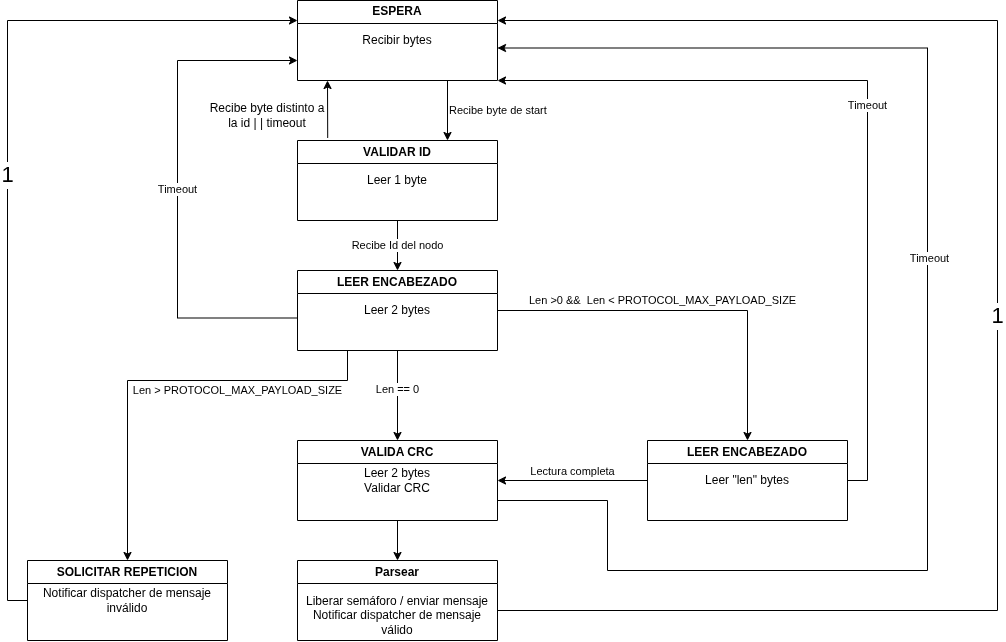
\includegraphics[width=1\textwidth]{img/MEF_Ramodbus.png}
	\caption{Máquina de estados finitos del parser del protocolo.}
	\label{fig:MEF_RAMODBUS}
\end{figure}


Cuando una tarea de algún módulo quiere mandar un dato debe utilizar la función composer. 
Esta recibe como argumentos el comando a enviar, la longitud del payload y un puntero a un buffer para los datos. Esto para no pasar la trama por copia, haciendo el transporte más eficiente. Esto conlleva un riesgo por lo que se añade como argumento un semáforo que bloquee la escritura de este.

Para la comunicación entre el composer y el dispacher se utiliza una cola de mensajes, ideal para transmitir estructuras como las creadas para el protocolo:

\begin{lstlisting}
	typedef struct {
		
		uint8_t id;
		uint8_t cmd;
		uint8_t len;
		uint8_t *payload;
		uint16_t CRC;
	} msj_t;
	
	typedef struct {
		
		msj_t msj;
		SemaphoreHandle_t semaforo;
	} q_msj_t;
\end{lstlisting}

La estructura de cola \textit{q\_msj\_t} contiene al semáforo y a una variable de la estructura \textit{msj\_t}. La función calcula el CRC en base a los datos recibidos y llena la estructura para encolarla. Previamente, si se utilizó un semáforo, lo toma para proteger al buffer de ser modificado durante la transmisión.


La tarea dispatcher es la encargada de llamar a la función (en este caso \texttt{app\_uart\_send}) que transmite los mensajes. Esta guarda el mensaje en un buffer y lo envía mediante la función descripta anteriormente

La tarea dispatcher es la encargada de llamar a la función (en este caso \texttt{app\_\allowbreak uart\_\allowbreak send}) que transmite los mensajes. Esta guarda el mensaje en un buffer y lo envía mediante la función descripta anteriormente

La tarea se mantiene bloqueada hasta recibir una notificación del parser, es decir solo transmite en respuesta a las encuestas. En el caso de que la notificación sea de fallo transmite un comando de NACK. En el caso de que la notificación sea de aviso de mensaje válido, va a revisar si en la cola del composer hay datos en espera que transmitir, para armar el mensaje y enviarlo. Luego de enviarlo libera el semáforo para permitir la reescritura del buffer de datos. En caso de que no haya datos en cola, construye y envía un comando de ACK.

Esto indica dos cosas importantes de comportamiento del protocolo:
Primero que, dada la alta prioridad que deben tener las tareas de este respecto a las demás de la aplicación para mantener la fluidez, lo más probable es que la respuesta a cualquier comando siempre sea un ACK y que los datos esperados se transmitan en un ciclo de polling siguiente.

Lo siguiente es que los datos se transmiten en orden de llegada, este orden vendrá dado en la aplicación por la  prioridad que se le asigne a cada tarea.

\begin{figure}[h]
	\centering
	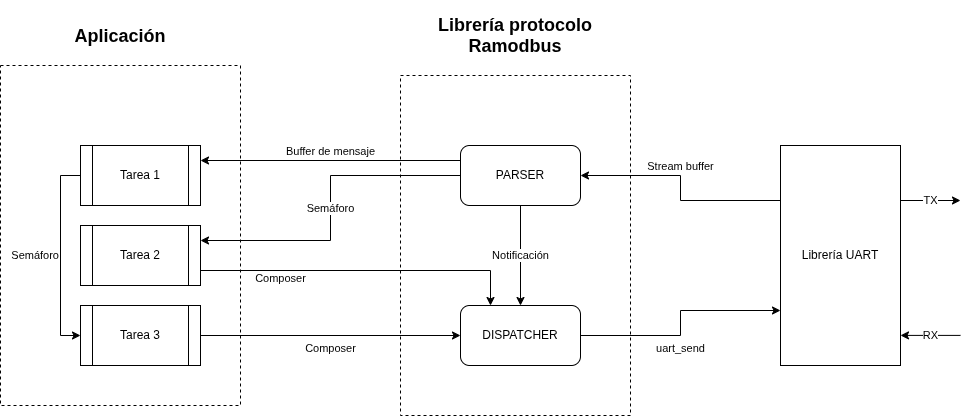
\includegraphics[width=1\textwidth]{img/RAMODBUS.png}
	\caption{Esquema de operación del protocolo}
	\label{fig:RAMODBUS}
\end{figure}

Si bien a cada comando (exceptuando los dos primeros) se le corresponde una tarea, esto no necesariamente se cumple en el sentido inverso. No todas las tareas tiene que devolver confirmaciones. Además, puede que haya tareas que encolen datos, pero que reaccionen no a un comando de un protocolo sino a cualquier otro evento, como una interrupción o la orden de otra tarea.

\subsubsection{Tareas reactivas al protocolo}
La estructura de una tarea que reacciona a un comando del protocolo es, en principio,  sencilla. Durante la inicialización obtiene, mediante la función getter correspondiente, el semáforo binario o message buffer asociado al comando y verifica que la operación haya sido exitosa. Luego entra en un bucle infinito en el que permanece bloqueada indefinidamente hasta recibir un mensaje o liberarse el semáforo. Una vez desbloqueada, ejecuta la acción correspondiente y vuelve al estado bloqueado al finalizar. Como ejemplo, la tarea que implementa el comando obligatorio de reinicio se muestra a continuación.

\begin{minipage}{\linewidth}
\begin{lstlisting}[frame=single]
    void reset_task(void *pvParameters) {
    
    SemaphoreHandle_t cmd_sem = protocol_get_ctrl_sem(CMD_RESET);
    if (cmd_sem == NULL) {
        ESP_LOGE("RESET", "No se pudo obtener el semaforo de reset");
        esp_restart();
    }

    while(1){
        if (xSemaphoreTake(cmd_sem, portMAX_DELAY) == pdTRUE) {
            esp_restart();
        }                               
    }
}
\end{lstlisting}
\end{minipage}

\subsubsection{Manejo de entradas y salidas digitales}

Este módulo implementa el control de las dos salidas digitales del controlador, correspondientes al relé de apertura de la puerta y al relé del timbre, además de la lectura de la entrada digital asociada al pulsador del timbre.

Durante la inicialización se configuran los pines de entrada y salida, se obtienen mediante la API del protocolo los semáforos correspondientes a los comandos de apertura de puerta y captura de fotografía, y se crea un temporizador de software utilizado para controlar la duración del accionamiento del relé del timbre.

La apertura de la puerta se implementa mediante una tarea reactiva al protocolo. Esta permanece bloqueada sobre el semáforo asociado al comando correspondiente y, al recibir la orden, activa el relé durante un tiempo configurable. Antes de volver al estado de espera envía la confirmación de ejecución mediante el protocolo de comunicaciones.

La detección de la pulsación del timbre se realiza mediante una interrupción externa configurada sobre el flanco descendente de la señal. Cuando esta ocurre, el manejador de interrupción libera el semáforo asociado a la captura de fotografías para despertar la tarea correspondiente y activa el relé del timbre. Como las rutinas de interrupción deben ejecutarse en el menor tiempo posible, la desactivación del relé no se realiza desde la propia interrupción sino mediante un temporizador de software, cuyo callback se ejecuta una vez transcurrido el tiempo programado.

Esta arquitectura permite minimizar el tiempo de ejecución de la rutina de interrupción, delegando el procesamiento de mayor duración a las tareas del sistema operativo y a los mecanismos de temporización provistos por FreeRTOS.

\subsubsection{Módulo de Identificación NFC}

Para la lectura de credenciales de acceso, se implementó un módulo basado en el transceptor PN532. La elección de este integrado radica en su amplia compatibilidad con protocolos RFID a 13.56 MHz, en particular la norma ISO/IEC 14443A, lo cual permite interactuar fluidamente con etiquetas de la familia NTAG21x (NTAG213, NTAG215 y NTAG216). 



El control del chip se resolvió integrando el componente de software libre \enquote{\texttt{garag\_\_esp-idf-pn532}}. Esta biblioteca abstrae la comunicación SPI de bajo nivel y proporciona una API para la inicialización del controlador, la configuración de sus temporizadores y el envío de comandos al circuito integrado PN532.

El funcionamiento del módulo está gestionado por el RTOS mediante la creación de tres tareas concurrentes: \textit{Lectora}, \textit{Programadora} y \textit{Arbitro}.

El sistema opera bajo dos estados mutuamente excluyentes: Modo Lectura y Modo Programación. Dado que ambas tareas (\textit{nfc\_task} y \textit{nfc\_config\_task}) compiten por el uso del mismo periférico SPI y el mismo handler del PN532, se implementó un mecanismo de exclusión donde una tarea suspende a la otra (\textit{vTaskSuspend} y \textit{vTaskResume}) según el estado dictaminado por la tarea de arbitraje. 

El árbitro, a su vez, reacciona directamente a las peticiones del coordinador central. Utiliza un semáforo binario cedido por maestro para alternar el estado. Si se recibe el comando de programación (\textit{CMD\_PROGMODE}), el sistema entra en una ventana de tiempo limitada (\textit{timeout}) para configurar una nueva etiqueta. Si no se detecta actividad o finaliza el tiempo, el sistema retorna de forma segura a su estado natural de lectura, garantizando la operatividad ininterrumpida del control de acceso.


Uno de los mayores desafíos en sistemas de identificación por radiofrecuencia es la mitigación de ataques de clonación y repetición. Para abordar esto, el sistema no se limita a leer el UID (Identificador Único) de 7 bytes de la tarjeta, sino que implementa un esquema de autenticación dinámica y contadores de lectura.

Durante el modo de programación, al detectar una tarjeta NTAG virgen, el sistema ejecuta una función de derivación de claves utilizando HMAC-SHA256 (mediante la librería \textit{mbedtls}). Se utiliza una clave maestra residente en el firmware del equipo y el UID único de la tarjeta para generar un hash de 32 bytes. Los primeros 6 bytes de este hash se truncan y se inyectan en la memoria de la NTAG para configurar el \textit{Password} (PWD) de 4 bytes y el \textit{Password Acknowledge} (PACK) de 2 bytes. 

De esta forma, cada credencial del sistema posee una contraseña única matemáticamente vinculada a su hardware que se calcula en el acto, evitando la vulnerabilidad de alojar contraseñas en una base de datos.

Adicionalmente, se configuran los registros de control de la NTAG para activar la función \textit{ASCII Mirror}. Esta característica escribe automáticamente el valor actual de un contador de interacciones interno de la etiqueta en la memoria de usuario cada vez que la tarjeta es energizada por el campo de radiofrecuencia.

\begin{table}[H]
    \centering
    \begin{tabular}{@{}c c c c c c@{}}
        \toprule
        \textbf{Página (Hex)} & \textbf{Byte 0} & \textbf{Byte 1} & \textbf{Byte 2} & \textbf{Byte 3}  \\
        \midrule
        \texttt{0x29/0x83/0xE3} & \texttt{MIRROR} & \texttt{RFUI} & \texttt{MIRROR\_PAGE} & \texttt{AUTH0}  \\
        \texttt{0x2A/0x84/0xE4} & \texttt{ACCES}  & \texttt{RFUI} & \texttt{RFUI} & \texttt{RFUI}  \\
        \texttt{0x2B/0x85/0xE5} & \texttt{PWD0}   & \texttt{PWD1} & \texttt{PWD2} & \texttt{PWD3}  \\
        \texttt{0x2C/0x86/0xE6} & \texttt{PACK0}  & \texttt{PACK1}& \texttt{RFUI} & \texttt{RFUI}  \\
        \bottomrule
    \end{tabular}
    \caption{Mapa de configuración de registros de seguridad y espejado en familia NTAG213/215/216.}
    \label{tab:ntag_registers}
\end{table}

El byte MIRROR contiene las configuraciones del espejado ASCII,  se configura con el valor 0x85  Los dos bits más significativos indican que el espejado se realizará sobre el contador al configurarse como. Los siguientes dos indican en que posición de la página seleccionada sé  comienza a escribir el dato, en este caso al principio. El bit 2 es la habilitación de modulación fuerte, la cual se deja por defecto en 1 mientras que los demás bits están reservados y se mantienen en 0.

Todos los bytes notados \enquote{RFUI} son de reserva y se mantienen en su valor por defecto 0x00.
El byte MIRROR\_ PAGE determina en que página se escribirá el espejo contador.
El byte AUTH0 define a partir de qué página se protegen los datos con contraseña, el valor por defecto es 0xFF, es decir que se permite la lectoescritura de todas las páginas, lo habitual es configurarlo en 0x04, es decir dejar libres las páginas de información de fábrica y proteger el resto.

El byte ACCES se configura con el valor 0x98, el cual si se analiza  bit a bit indica que la contraseña protege contra escritura y lectura, y que el contador está activado. Además, permite establecer un número máximo de intentos de lectura y activar un bloqueo permanente del tag. Estas opciones se descartaron por el riesgo de dejarlo inutilizado accidentalmente.

La página PWD guarda la contraseña del tag, aquí se escribe el password de 4 bytes calculado mediante el hash. La página PACK contiene los dos bytes de confirmación de la autenticación con contraseña que también se calcula mediante el hash.




En su régimen nominal de lectura, el flujo de ejecución sigue una estricta secuencia de validación. Al acercar una tarjeta, se lee su UID y se calcula localmente el hash esperado. Posteriormente, se envía un comando de autenticación al PN532 pasándole la contraseña calculada (\textit{NTAG\_COMMAND\_PWD\_AUTH}). Si la NTAG devuelve el PACK correcto, se confirma la legitimidad de la tarjeta.

Superada la barrera de seguridad, se emite un comando de lectura rápida (\textit{NTAG\_COMMAND\_FAST\_READ}) apuntando a la dirección configurada previamente para el \textit{Mirror}. El valor retornado, que representa el contador de lecturas en formato de caracteres hexadecimales ASCII, es convertido a un entero de 32 bits (\textit{strtoul}). 

Finalmente, la información a reportar se condensa en un \textit{payload} de 10 bytes: los 7 bytes correspondientes al UID físico de la tarjeta, seguidos de 3 bytes que representan el valor del contador dinámico. Este bloque de datos se despacha mediante la función \textit{composer} de Ramodbus bajo el comando \textit{CMD\_NFC}, sincronizando el envío mediante un semáforo para asegurar la integridad de la memoria compartida hasta que el despachador de la capa de red confirme su transmisión hacia el servidor.

Se puede, mediante un comando de las NTAG, acceder al valor del contador de forma directa, sin tener que leer un registro ni convertirlo desde ASCII a un número, pero este comando no aumenta el contador como una lectura, por lo que para usarlo debería realizarse una lectura a un registro cualquiera, lo cual agrega puntos de falla en la comunicación del tag con el módulo.